%%%%%%%%%%%%%%%%%%%%%%%%%%%%%%%%%%%%%%%%%%%%%%%%%%%%%%%%%%%%%%%%%%%%%%
\section{Vision générale du projet ALORA}
%%%%%%%%%%%%%%%%%%%%%%%%%%%%%%%%%%%%%%%%%%%%%%%%%%%%%%%%%%%%%%%%%%%%%%

Le projet ALORA (\textit{Automatic Learning for Oral Resource-poor African Languages})
a pour ambition de proposer une méthodologie générale permettant de développer
progressivement des ressources numériques pour les langues orales peu dotées.

Plutôt que de commencer par la construction d'un modèle de traduction ou d'un
assistant conversationnel, l'approche proposée consiste à reproduire, autant
que possible, les grandes étapes de l'apprentissage d'une langue.

Autrement dit, avant d'espérer comprendre ou générer une langue, un système
d'intelligence artificielle doit d'abord apprendre à écouter, observer,
identifier les régularités de la parole, construire progressivement une
représentation interne de la langue, puis exploiter cette connaissance pour
développer des outils linguistiques.

Cette vision conduit naturellement à une architecture organisée en plusieurs
phases complémentaires.

%%%%%%%%%%%%%%%%%%%%%%%%%%%%%%%%%%%%%%%%%%%%%%%%%%%%%%%%%%%%%%%%%%%%%%

\subsection{Vision globale}

\begin{figure}[H]
\centering

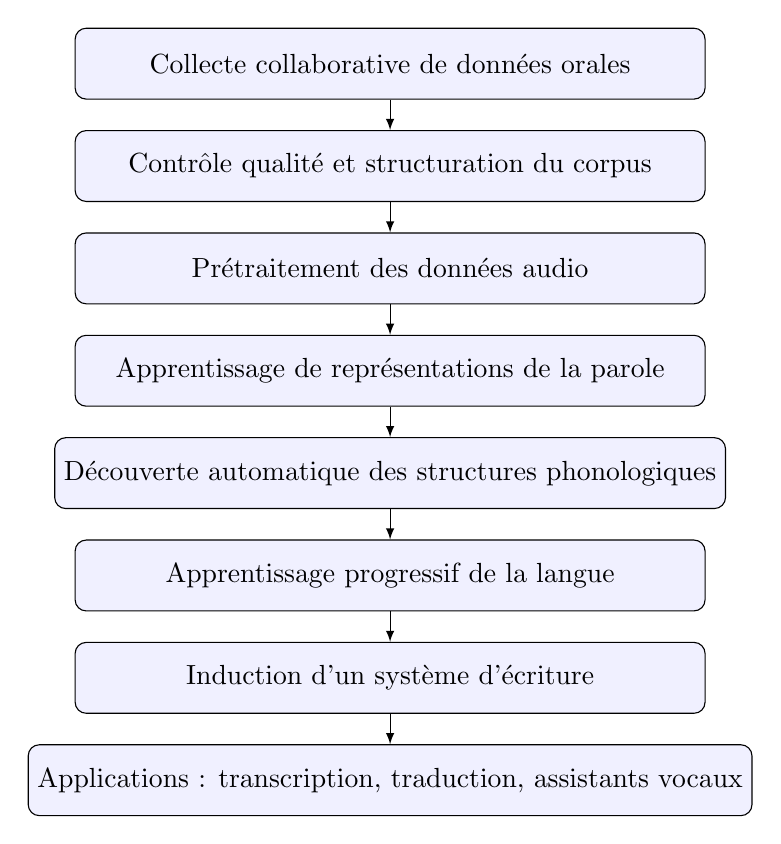
\begin{tikzpicture}[
node distance=1.3cm,
every node/.style={
draw,
rounded corners,
align=center,
minimum width=8cm,
minimum height=0.9cm,
fill=blue!6
},
>=latex
]

\node (collecte) {Collecte collaborative de données orales};

\node (qualite) [below of=collecte]
{Contrôle qualité et structuration du corpus};

\node (prep) [below of=qualite]
{Prétraitement des données audio};

\node (speech) [below of=prep]
{Apprentissage de représentations de la parole};

\node (phono) [below of=speech]
{Découverte automatique des structures phonologiques};

\node (langue) [below of=phono]
{Apprentissage progressif de la langue};

\node (alphabet) [below of=langue]
{Induction d'un système d'écriture};

\node (applications) [below of=alphabet]
{Applications : transcription, traduction, assistants vocaux};

\draw[->] (collecte)--(qualite);
\draw[->] (qualite)--(prep);
\draw[->] (prep)--(speech);
\draw[->] (speech)--(phono);
\draw[->] (phono)--(langue);
\draw[->] (langue)--(alphabet);
\draw[->] (alphabet)--(applications);

\end{tikzpicture}

\caption{Vision générale du projet ALORA}
\end{figure}

%%%%%%%%%%%%%%%%%%%%%%%%%%%%%%%%%%%%%%%%%%%%%%%%%%%%%%%%%%%%%%%%%%%%%%

\subsection{Principe général}

Contrairement aux approches classiques qui supposent l'existence d'une langue
déjà écrite et de nombreuses ressources annotées, ALORA cherche à construire
ces ressources progressivement.

Le projet débute donc par la création d'un corpus oral de qualité, obtenu grâce
à une collecte collaborative auprès de locuteurs natifs.

Une fois ce corpus constitué, plusieurs traitements successifs permettront de
préparer les données pour l'apprentissage automatique :

\begin{itemize}

\item nettoyage des enregistrements ;

\item normalisation des formats audio ;

\item organisation des métadonnées ;

\item contrôle qualité ;

\item préparation du corpus pour les futurs modèles.

\end{itemize}

Ces premières étapes constituent les fondations du projet. Elles conditionnent
directement la qualité des modèles développés par la suite.

%%%%%%%%%%%%%%%%%%%%%%%%%%%%%%%%%%%%%%%%%%%%%%%%%%%%%%%%%%%%%%%%%%%%%%

\subsection{Une progression par niveaux}

L'objectif n'est pas de résoudre simultanément tous les problèmes liés à une
langue peu dotée.

Au contraire, ALORA adopte une stratégie incrémentale.

Chaque étape produit des résultats exploitables qui servent de base à la
suivante.

\begin{center}

\begin{tabular}{cl}

\toprule

Niveau & Objectif principal \\

\midrule

1 & Construire un corpus oral fiable \\

2 & Préparer les données pour l'apprentissage \\

3 & Apprendre des représentations de la parole \\

4 & Identifier automatiquement les unités phonologiques \\

5 & Comprendre progressivement la structure de la langue \\

6 & Étudier la possibilité de proposer une représentation écrite \\

7 & Développer des applications linguistiques \\

\bottomrule

\end{tabular}

\end{center}

Cette progression permet de limiter les risques scientifiques tout en produisant
des résultats exploitables dès les premières phases du projet.

%%%%%%%%%%%%%%%%%%%%%%%%%%%%%%%%%%%%%%%%%%%%%%%%%%%%%%%%%%%%%%%%%%%%%%

\subsection{Positionnement du travail proposé}

La totalité de cette vision représente un projet de recherche pouvant
s'étendre sur plusieurs années.

Le travail envisagé durant l'été ne constitue donc que la première étape de
cette feuille de route.

L'objectif est de construire des bases suffisamment solides pour permettre le
développement des étapes suivantes dans le cadre du semestre S5, puis du Projet
de Fin d'Études (PFE).

À ce stade, les questions relatives à la découverte automatique des unités
phonologiques, à l'apprentissage de la langue ou encore à l'induction d'un
système d'écriture restent ouvertes. Elles feront l'objet d'une étude
progressive au fur et à mesure de l'avancement du projet.

\begin{objectif}

L'objectif principal de cette première phase n'est pas de développer un modèle
d'intelligence artificielle performant, mais de concevoir une méthodologie de
collecte et d'organisation des données suffisamment robuste pour servir de
fondation à l'ensemble du projet ALORA.

\end{objectif}